\documentclass{diss}
\usepackage{mymacros}

\usepackage{tikz,pgflibraryshapes}
\usetikzlibrary{arrows, calc, decorations.pathmorphing,circuits.ee.IEC}
\usetikzlibrary{shapes.misc, fit}

\usepackage[psfixbb,graphics,tightpage,active]{preview}
\PreviewEnvironment{tikzpicture}

\begin{document}
%%%%%%%%%%%%%%%%%%%%%%%%%%%%%%%%%%%%%%%%%%%%%%%%%%%%%%%%%%%%%%%%%%%%%%%%%%%%%%%%

\begin{tikzpicture}[
  circuit ee IEC,
  x=1cm,
  y=1cm
]

\tikzstyle{nl}=[fill=white,inner sep=1pt,outer sep=0,opacity=0.8];

\node[inner sep=0, outer sep=0] (fig) at (0,0)
{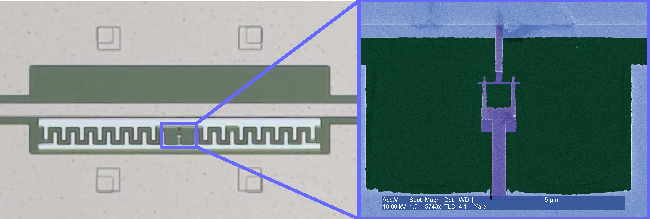
\includegraphics{transmon_photo}};

%\draw[step=1.0,gray,very thin] (-6,-2) grid (5,2); % background grid
%\draw (0,0) circle (3pt);

\node[nl] at (-4.5, -1.25) {\footnotesize 1};
\node[nl] at (-3.95, -0.6) {\footnotesize 2};
\node[nl] at (-3.5, -0.3)  {\footnotesize 3};
\node[nl] at (-5.0, 0)     {\footnotesize 4};
\node[nl] at (-4.5, +1.25) {\footnotesize 5};
\node[nl] at (2.95, 0.225) {\footnotesize 6};
\node [contact] (contact-top)    at (-5.4,0) {};
\node [contact] (contact-bottom) at (-5.4,-1) {};
\draw (contact-top) -- ++(-0.5,0)
      to [voltage source={info'=$U$}] ++(0,-1)
      -- (contact-bottom);

\draw[|-|] (-3.6,-1.3) -- node[midway,below]{\small $\SI{100}{\micro\metre}$} +(2.3,0);


\end{tikzpicture}
%%%%%%%%%%%%%%%%%%%%%%%%%%%%%%%%%%%%%%%%%%%%%%%%%%%%%%%%%%%%%%%%%%%%%%%%%%%%%%%%

\end{document}
